% Options for packages loaded elsewhere
\PassOptionsToPackage{unicode}{hyperref}
\PassOptionsToPackage{hyphens}{url}
\documentclass[
]{article}
\usepackage{xcolor}
\usepackage[margin=1in]{geometry}
\usepackage{amsmath,amssymb}
\setcounter{secnumdepth}{-\maxdimen} % remove section numbering
\usepackage{iftex}
\ifPDFTeX
  \usepackage[T1]{fontenc}
  \usepackage[utf8]{inputenc}
  \usepackage{textcomp} % provide euro and other symbols
\else % if luatex or xetex
  \usepackage{unicode-math} % this also loads fontspec
  \defaultfontfeatures{Scale=MatchLowercase}
  \defaultfontfeatures[\rmfamily]{Ligatures=TeX,Scale=1}
\fi
\usepackage{lmodern}
\ifPDFTeX\else
  % xetex/luatex font selection
\fi
% Use upquote if available, for straight quotes in verbatim environments
\IfFileExists{upquote.sty}{\usepackage{upquote}}{}
\IfFileExists{microtype.sty}{% use microtype if available
  \usepackage[]{microtype}
  \UseMicrotypeSet[protrusion]{basicmath} % disable protrusion for tt fonts
}{}
\makeatletter
\@ifundefined{KOMAClassName}{% if non-KOMA class
  \IfFileExists{parskip.sty}{%
    \usepackage{parskip}
  }{% else
    \setlength{\parindent}{0pt}
    \setlength{\parskip}{6pt plus 2pt minus 1pt}}
}{% if KOMA class
  \KOMAoptions{parskip=half}}
\makeatother
\usepackage{longtable,booktabs,array}
\usepackage{calc} % for calculating minipage widths
% Correct order of tables after \paragraph or \subparagraph
\usepackage{etoolbox}
\makeatletter
\patchcmd\longtable{\par}{\if@noskipsec\mbox{}\fi\par}{}{}
\makeatother
% Allow footnotes in longtable head/foot
\IfFileExists{footnotehyper.sty}{\usepackage{footnotehyper}}{\usepackage{footnote}}
\makesavenoteenv{longtable}
\usepackage{graphicx}
\makeatletter
\newsavebox\pandoc@box
\newcommand*\pandocbounded[1]{% scales image to fit in text height/width
  \sbox\pandoc@box{#1}%
  \Gscale@div\@tempa{\textheight}{\dimexpr\ht\pandoc@box+\dp\pandoc@box\relax}%
  \Gscale@div\@tempb{\linewidth}{\wd\pandoc@box}%
  \ifdim\@tempb\p@<\@tempa\p@\let\@tempa\@tempb\fi% select the smaller of both
  \ifdim\@tempa\p@<\p@\scalebox{\@tempa}{\usebox\pandoc@box}%
  \else\usebox{\pandoc@box}%
  \fi%
}
% Set default figure placement to htbp
\def\fps@figure{htbp}
\makeatother
\setlength{\emergencystretch}{3em} % prevent overfull lines
\providecommand{\tightlist}{%
  \setlength{\itemsep}{0pt}\setlength{\parskip}{0pt}}
\usepackage{titlesec}
\titleformat{\section}{\centering\normalfont\Large\bfseries}{\thesection}{1em}{}
\titleformat{\subsection}{\centering\normalfont\large\bfseries}{\thesubsection}{1em}{}
\titleformat{\subsubsection}{\centering\normalfont\normalsize\bfseries}{\thesubsubsection}{1em}{}

\usepackage{silence}
\WarningsOff*
\usepackage{booktabs}
\usepackage{longtable}
\usepackage{array}
\usepackage{multirow}
\usepackage{wrapfig}
\usepackage{float}
\usepackage{colortbl}
\usepackage{pdflscape}
\usepackage{tabu}
\usepackage{threeparttable}
\usepackage{threeparttablex}
\usepackage[normalem]{ulem}
\usepackage{makecell}
\usepackage{xcolor}
\usepackage{bookmark}
\IfFileExists{xurl.sty}{\usepackage{xurl}}{} % add URL line breaks if available
\urlstyle{same}
\hypersetup{
  pdftitle={ANALISIS DEL NIVEL EDICATIVO DE LOS PADRES Y EL TIPO DE ALIMENTACION DE LOS ESTUDIANES COMO POSIBLES INDICADORES DEL RENDIMIENTO ACADEMICO DE LOS MISMOS MEDIANTE METODOS ESTADISTICOS},
  pdfauthor={David Mazza, Eros Bande, Sofia Rodriguez},
  hidelinks,
  pdfcreator={LaTeX via pandoc}}

\title{ANALISIS DEL NIVEL EDICATIVO DE LOS PADRES Y EL TIPO DE
ALIMENTACION DE LOS ESTUDIANES COMO POSIBLES INDICADORES DEL RENDIMIENTO
ACADEMICO DE LOS MISMOS MEDIANTE METODOS ESTADISTICOS}
\author{David Mazza, Eros Bande, Sofia Rodriguez}
\date{2025-03-17}

\begin{document}
\maketitle

\subsection{HIPOTESIS}\label{hipotesis}

La alimentación de los estudiantes y el nivel educativo de los padres
influye significativamente en el rendimiento académico de sus hijos, de
modo que, a mayor nivel educativo de los padres, mayor será el
rendimiento académico de los hijos.

\subsection{DESCRIPCION}\label{descripcion}

Esta investigación tiene como principal enfoque analizar como el nivel
educativo de los padres y la alimentación disponible para los
estudiantes se relaciona con los resultados de las calificaciones
obtenidas en tres exámenes distintos, tomando como base un grupo
representativo de colegiales estado unidenses con la finalidad de
presentar información concreta de los resultados obtenidos para que las
instituciones pertinentes diseñen planes de acción.

El rendimiento académico es uno de los pilares fundamentales del sistema
educativo, este no solo refleja las habilidades intelectuales
individuales de los alumnos, sino que también está influenciado por
factores externos, como el entorno familiar, el apoyo recibido y el
nivel educativo de los padres. Estudios previos han destacado el papel
de estas variables externas en la productividad académica de los
estudiantes.

En particular, el nivel educativo de los padres puede influir de
diversas maneras: fomentando una cultura de estudio, sirviendo como
modelo a seguir y brindando apoyo académico. Por otro lado, la
alimentación adecuada incide directamente en la capacidad de
concentración, un aspecto crucial para el éxito en cualquier ámbito
académico.

Aunque muchas personas podrían afirmar, por lógica o experiencia, que
estas variables influyen en el desempeño estudiantil, es fundamental
respaldar estas afirmaciones con indicadores y análisis estadísticos que
eliminen la subjetividad y las opiniones personales. Comprender esta
relación permitirá identificar áreas que requieren atención y diseñar
herramientas que favorezcan un entorno propicio para el rendimiento
académico.

\subsection{JUSTIFICACION}\label{justificacion}

El rendimiento académico de los estudiantes es un tema de gran
relevancia en el ámbito educativo, ya que está estrechamente vinculado a
oportunidades futuras y al desarrollo socioeconómico. Por ende,
identificar las variables que pueden predecir el rendimiento escolar es
de gran importancia para implementar soluciones efectivas, ya sea
mediante ayudas gubernamentales, campañas de concientización o programas
de apoyo específicos.

Diversos estudios han sugerido que el nivel educativo de los padres
puede ser un factor determinante en el éxito escolar de los hijos,
debido a la influencia que ejercen en la formación de hábitos de
estudio, la motivación y el acceso a recursos culturales, educativos y
alimenticios. Sin embargo, en el contexto local, existe una brecha en la
investigación que aborde esta relación de manera específica. Este
estudio busca contribuir a la comprensión de este fenómeno,
proporcionando información valiosa para diseñar políticas educativas y
estrategias que apoyen a las familias en la promoción del éxito
académico de sus hijos.

Un país con una educación sólida es sinónimo de progreso y desarrollo.
Para mejorar el sistema educativo, es necesario prestar atención a su
comportamiento de manera detallada y basada en información confiable, la
estadística se convierte así en la herramienta más efectiva para
lograrlo.

\subsection{OBJETIVOS}\label{objetivos}

\subsubsection{Objetivo general:}\label{objetivo-general}

\begin{itemize}
\tightlist
\item
  Analizar la relación entre el nivel educativo de los padres y la
  alimentación de los estudiantes con su desempeño académico en exámenes
  de habilidad verbal, matemática e inglés.
\end{itemize}

\subsubsection{Objetivos específicos:}\label{objetivos-especuxedficos}

\begin{itemize}
\item
  Realizar un análisis descriptivo de las variables nivel educativo de
  los padres, la alimentación de los estudiantes y las calificaciones de
  los estudiantes en los exámenes establecidos.
\item
  Establecer la relación entre el nivel educativo de los padres y los
  resultados de los estudiantes en los exámenes de habilidad verbal,
  matemática e inglés.
\item
  Determinar si la alimentación de los estudiantes está relacionada con
  el rendimiento académico en los exámenes mencionados.
\item
  Determinar cuál de las dos variables es más influyente en el desempeño
  escolar.
\end{itemize}

\subsection{VARIABLES}\label{variables}

\begin{itemize}
\tightlist
\item
  Nota en exámenes: Este es el principal indicador de desempeño
  académico y se expresa en los resultados de 3 distintas pruebas,
  matemáticas, lectura y escritura. Es una variable cuantitativa
  discreta
\item
  Nivel educativo de los padres: Es el nivel más alto de educación
  alcanzado por los responsables de los estudiantes. Este tendrá
  distintas categorías, como educación primaria, secundaria, superior,
  entre otros. Es una variable cualitativa ordinal. Esta variable consta
  de las categorías:

  \begin{itemize}
  \item
    Alguna educación secundaria (some high school): Indica que los
    padres no completaron la educación secundaria.
  \item
    Educación secundaria (high school): Se refiere a que los padres
    completaron la escuela secundaria, incluyendo aquellos que lo
    hicieron a través de programas de equivalencia como el GED.
  \item
    Alguna educación universitaria (some college): Se refiere a los
    padres que asistieron a la universidad, pero no obtuvieron un
    título. Esto puede incluir la obtención de créditos, diplomas o
    certificados.
  \item
    Título de asociado (associate's degree): Indica que los padres
    obtuvieron un título de asociado, que generalmente se obtiene en dos
    años en un colegio comunitario o escuela vocacional.
  \item
    Título de licenciatura o superior (Bachelor's \& Master's degree) :
    Significa que los padres completaron un programa de licenciatura
    (cuatro años o más) o incluso un nivel de educación superior, como
    una maestría o un doctorado.
  \end{itemize}
\item
  Almuerzo de los estudiantes: Se considera la calidad del almuerzo de
  los estudiantes en dos categorías, estándar y sin almuerzo o reducido.
  Es una variable cualitativa nominal

  \begin{itemize}
  \tightlist
  \item
    Sin almuerzo o reducido (free/reduced): Alimentación deficiente en
    la que se presentan carencias de nutrientes importantes en el
    desarrollo de una persona de edad temprana, que tiene consecuencias
    cognitivas a largo plazo
  \item
    Estándar (standard): Alimentación balanceada en la que se cumplen
    todas las necesidades básicas.
  \end{itemize}
\end{itemize}

Estas variables fueron seleccionadas porque representan factores
externos que, aunque no son elegidos por los estudiantes, tienen un gran
impacto en sus vidas. El nivel educativo de los padres y la alimentación
diaria son determinantes en las posibilidades académicas, recreativas y
alimenticias de un individuo, aspectos que, a su vez, pueden influir en
su rendimiento académico. Determinar si esto se cumple o no, será el
objetivo de esta investigación.

\subsection{LIMITES Y ALCANCE}\label{limites-y-alcance}

El límite de esta investigación recae en el alcance de la conclusión
establecida. Es decir, el enfoque principal del trabajo es establecer la
relación de las dos variables ya mencionadas con el desempeño
estudiantil, las razones específicas de el por qué esto sucede está más
allá del alcance de los datos disponibles.

\subsection{ANTECEDENTES}\label{antecedentes}

Un tema de gran interés global es el rendimiento escolar de los
estudiantes ya dado su relevancia en el crecimiento individual y, por
ende, su reflejo a nivel social. Existen diversos estudios que exploran
diferentes variables y como estos influyen en el desempeño escolar,
algunos de estos son el nivel educativo de los padres y la alimentación
de los estudiantes.

El nivel educativo de los padres puede influir de muchas maneras, un
artículo de la organización ClearingHouse (2020) realizó una síntesis de
estudios externos y determino que el comportamiento de los estudiantes
se moldea por la observación y experiencias formativas directas, es
decir, cuando los padres muestran un comportamiento orientado a logros
académicos, avance en carreras universitarias, postgrados,
investigaciones, y facilitan oportunidades de este tipo para sus hijos,
estos empiezan a creer en la importancia de este comportamiento y lo
priorizan.

Además, otro factor importante en el desempeño académico es la cantidad
de tiempo que pasan los estudiantes con sus padres, especialmente si es
de calidad y enfocado a desarrollar sus talentos. ClearingHouse (2020)
establece lo siguiente:

``Since children learn, in part, by observation, one of the key
components to a child's success is parental time investment (Kalil,
Ryan, \& Corey, 2012). Highly educated parents spend more time with
their children (Guryan, Hurst, \& Kearney, 2008) and spend that time
actively developing their children's talents and skills (Lareau, 2002)''

(Como los niños aprenden, en parte, por observación, uno de los
componentes claves para su éxito es la inversión de tiempo parental.
Padres altamente educados pasan más tiempo con sus hijos y enfocan ese
tiempo en desarrollar activamente sus talentos y habilidades. Traducción
propia)

Distintos estudios argumentan que el nivel educativo de los padres no
necesariamente tiene una relación directa con el desempeño estudiantil,
sin embargo, otros académicos concluyen que si tiene una influencia
notable en el tiempo que dedican a sus hijos y a su educación, a pesar
de que su tiempo podría ser enfocado en otras actividades laborales de
mayor remuneración.

``The level of parental education is correlated with the amount of time
spent with children and argue that more educated parents spend more time
with their children. For example, Guryan et al.~found that mothers with
a college education or higher spend more than 4 hours per week with
their children than mothers with lower education.'' Kantova, K. (2024)

(El nivel de educacion de los padres esta correlacionado con la cantidad
de tiempo invertido con sus hijos y argumenta que los padres más
educados pasan más tiempo con sus hijos. Por ejemplo, Guryan et al
encontró que las madres con una educación universitaria o mayor pasan
más de 4 horas por semana con sus hijos que las madres con menos
educación. Traducción propia)

Además, Kantova (2024) establece a través de numerosas citas y
referencias a otros académicos que el porcentaje de graduación de High
school (Preparatoria o bachillerato) es menor en individuos que
pertenencen a un nucleo familiar de bajo nivel educativo comparado a
aquellos de familias más educadas, específicamente, un 72\% a 87\%
respectivamente. Esto es sumamente preocupante a nivel económico y
social. Kantova (2024) establece:

``Belfield and Levin (2007) claim that high school graduation is a
doorway to economic self-sufficiency and civic engagement. Without a
high school diploma, people are more likely to earn a lower income and
be arrested, which leads to higher costs for the US.'' (Belfield y Levin
(2007) afirman que graduarse de preparatoria es una puerta a la
autosuficiencia económica y el compromiso cívico. Sin un diploma de
preparatoria, las personas son más propensas a tener un menor ingreso
económico y a ser arrestar, lo que causa mayor costo para Estados
Unidos. Traducción propia)

Por otra parte, la fundación Amhersth Wilder Foundation explica la
importancia de una buena alimentación en el desarrollo integral de los
niños, proceso social y académico. Se ha demostrado que una alimentación
pobre o reducida afecta la capacidad de pensamiento, conducta y salud,
factores que influencia el desempeño estudiantil (Wilder Research, 2014)

Se han realizado numerosos estudios sobre este tema, prohibir comida
chatarra en campañas escolares y ofrecer alternativas más saludables en
las comidas. Esta investigación encontró que los estudiantes de las
escuelas donde se implementó esta idea tuvieron mejores calificaciones
en algunas materias comparado a quienes no estuvieron involucrados en el
experimento (Belot \& Jamesm 2009, como se citó en Wilder research,
2014)

Una nutrición balanceada, que satisfaga todas las necesidades
alimenticias de los estudiantes no solo evita enfermedades que afecten
la asistencia y desempeño escolar, también les da más energías a los
estudiantes, aumenta su concentración e incluso promueve su capacidad
cognitiva. (Bellisle, 2004; Sorhaindo \& Feinstein, 2006, como se citó
en Wilder research, 2014)

Malki, A (2018) realizó un estudio titulado ``Effects of Student
Nutrition on Academic Perfomance'' (Efectos de la nutrición escolar en
el desempeño academico) y determinó que los estudiantes que tenían una
situación de inseguridad alimenticia tenían una tendencia a un desempeño
escolar menor comparado con los demás, aquellos que consumían 2 comidas
por día tenían una tendencia a un rendimiento medio y los que tenían
acceso a comidas saludables y balanceadas, en promedio, tenían mejor
rendimiento. Esto fue determinado a través de un análisis de regresión
lineal.

A continuación, se mostraran los calculos descriptivos de la variable
cuantitativa llamada Desempeño, esta es sera utilizada como la sintesis
del desempeño escolar de los estudiantes

\begin{longtable}[]{@{}
  >{\centering\arraybackslash}p{(\linewidth - 16\tabcolsep) * \real{0.1176}}
  >{\centering\arraybackslash}p{(\linewidth - 16\tabcolsep) * \real{0.1059}}
  >{\centering\arraybackslash}p{(\linewidth - 16\tabcolsep) * \real{0.1176}}
  >{\centering\arraybackslash}p{(\linewidth - 16\tabcolsep) * \real{0.1412}}
  >{\centering\arraybackslash}p{(\linewidth - 16\tabcolsep) * \real{0.0941}}
  >{\centering\arraybackslash}p{(\linewidth - 16\tabcolsep) * \real{0.1176}}
  >{\centering\arraybackslash}p{(\linewidth - 16\tabcolsep) * \real{0.1176}}
  >{\centering\arraybackslash}p{(\linewidth - 16\tabcolsep) * \real{0.0941}}
  >{\centering\arraybackslash}p{(\linewidth - 16\tabcolsep) * \real{0.0941}}@{}}
\caption{Cálculo de medidas descriptivas}\tabularnewline
\toprule\noalign{}
\begin{minipage}[b]{\linewidth}\centering
Promedio
\end{minipage} & \begin{minipage}[b]{\linewidth}\centering
Mediana
\end{minipage} & \begin{minipage}[b]{\linewidth}\centering
Varianza
\end{minipage} & \begin{minipage}[b]{\linewidth}\centering
D.Estandar
\end{minipage} & \begin{minipage}[b]{\linewidth}\centering
CV
\end{minipage} & \begin{minipage}[b]{\linewidth}\centering
Kurtosis
\end{minipage} & \begin{minipage}[b]{\linewidth}\centering
Simetria
\end{minipage} & \begin{minipage}[b]{\linewidth}\centering
Minimo
\end{minipage} & \begin{minipage}[b]{\linewidth}\centering
Maximo
\end{minipage} \\
\midrule\noalign{}
\endfirsthead
\toprule\noalign{}
\begin{minipage}[b]{\linewidth}\centering
Promedio
\end{minipage} & \begin{minipage}[b]{\linewidth}\centering
Mediana
\end{minipage} & \begin{minipage}[b]{\linewidth}\centering
Varianza
\end{minipage} & \begin{minipage}[b]{\linewidth}\centering
D.Estandar
\end{minipage} & \begin{minipage}[b]{\linewidth}\centering
CV
\end{minipage} & \begin{minipage}[b]{\linewidth}\centering
Kurtosis
\end{minipage} & \begin{minipage}[b]{\linewidth}\centering
Simetria
\end{minipage} & \begin{minipage}[b]{\linewidth}\centering
Minimo
\end{minipage} & \begin{minipage}[b]{\linewidth}\centering
Maximo
\end{minipage} \\
\midrule\noalign{}
\endhead
\bottomrule\noalign{}
\endlastfoot
67.77 & 68.33 & 203.27 & 14.26 & 21.04\% & 0.11 & -0.3 & 9 & 100 \\
\end{longtable}

En la tabla 1 se presentan distintos cálculos sobre el comportamiento de
la variable cuantitativa ``Desempeño''. A continuación, se interpretarán
estos resultados para conocer a profundidad cómo se comportan las
calificaciones de los estudiantes.

El primer cálculo es el promedio de calificaciones cuyo valor es de
67,77 puntos. Esto significa que, en general, los estudiantes obtuvieron
una calificación promedio cercano a este valor. Luego, la mediana es de
68,33 puntos, este valor simboliza que el 50\% de los estudiantes tiene
una calificación por debajo a ese número y el otro 50\% por encima.

El valor de la varianza es de 203,27 puntos al cuadrado, al ser las
calificaciones entre 1 y 100 este valor es alto lo cual indica que hay
una dispersión significativa en las notas (algunos obtuvieron
calificaciones mucho más altas o más bajas que la media), en resumen,
las calificaciones presentan una gran heterogeneidad, es decir, no son
parecidas.

Una manera más sencilla de ver lo antes mencionado es con la desviación
estándar, su valor es de 14,26, lo cual significa que, en promedio, las
notas de los estudiantes se desvían en 14,26 puntos por encima o por
debajo de la media.

El coeficiente de variación indica cuanto representa la desviación
estándar en relación con la media, en este caso su valor es de 21,04\% y
es moderado, la desviación estándar es el 21,04\% del promedio. Las
notas no están ni muy concentradas ni muy dispersas.

Para saber la forma de la distribución de las notas, es necesario
interpretar el valor de 0,11 de kurtosis, esto significa que la mayoría
de las calificaciones están concentradas alrededor de la media y los
valores extremos, ya sean muy bajos como muy altos no son tan
frecuentes.

El valor -0,3 de la simetría indica que hay un ligero sesgo hacia la
izquierda, es decir, hay más estudiantes con calificaciones
significativamente más bajas al promedio que altas.

Por ultimo de esta tabla, la calificación mínima obtenida por algún
estudiante es de 9 y la máxima es de 100, una calificación perfecta.

En el siguiente grafico se puede observar la forma de la curva que
representa la concentración de los datos respecto al promedio

\begin{center}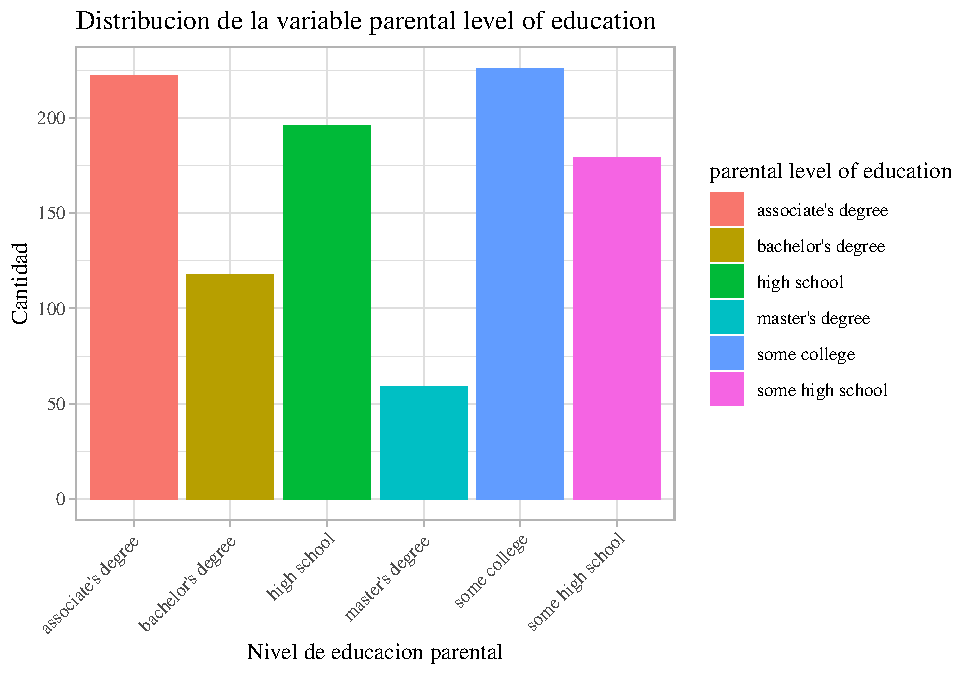
\includegraphics{Trabajo-Grupo-6.-Students-performance_files/figure-latex/unnamed-chunk-2-1} \end{center}

Estas son las distribuciones de las variables cualitativas, en cantidad
total, proporcion y graficos que faciliten su comprensión

\begin{longtable}[]{@{}ccc@{}}
\caption{Distribución de la variable parental level of
education}\tabularnewline
\toprule\noalign{}
parental level of education & Cantidad1 & Proporcion1 \\
\midrule\noalign{}
\endfirsthead
\toprule\noalign{}
parental level of education & Cantidad1 & Proporcion1 \\
\midrule\noalign{}
\endhead
\bottomrule\noalign{}
\endlastfoot
associate's degree & 222 & 22.2 \\
bachelor's degree & 118 & 11.8 \\
high school & 196 & 19.6 \\
master's degree & 59 & 5.9 \\
some college & 226 & 22.6 \\
some high school & 179 & 17.9 \\
\end{longtable}

En la tabla 2 se puede apreciar la distribución de la variable parental
level of education (Nivel de educación de los padres). Hay 222 (22,2\%)
padres con un nivel educativo con un associate's degree, 118 (11,8\%)
padres con un bachelor's degree, 196 (19,6) con high school, 59 con
master's degree (5,9), 226 (22,6) some college y finalmente, 179 (17,9)
some high school.

\begin{longtable}[]{@{}ccc@{}}
\caption{Distribución de la variable lunch}\tabularnewline
\toprule\noalign{}
lunch & Cantidad2 & Proporcion2 \\
\midrule\noalign{}
\endfirsthead
\toprule\noalign{}
lunch & Cantidad2 & Proporcion2 \\
\midrule\noalign{}
\endhead
\bottomrule\noalign{}
\endlastfoot
free/reduced & 355 & 35.5 \\
standard & 645 & 64.5 \\
\end{longtable}

En la tabla 3, al igual que la tabla 2 se expresa la distribución de una
variable, en este caso, la variable lunch (almuerzo). Hay 355 (35,5\%)
estudiantes cuyo almuerzo es reducido y 645 estudiantes (64,5\%) con un
almuerzo estándar.

\begin{center}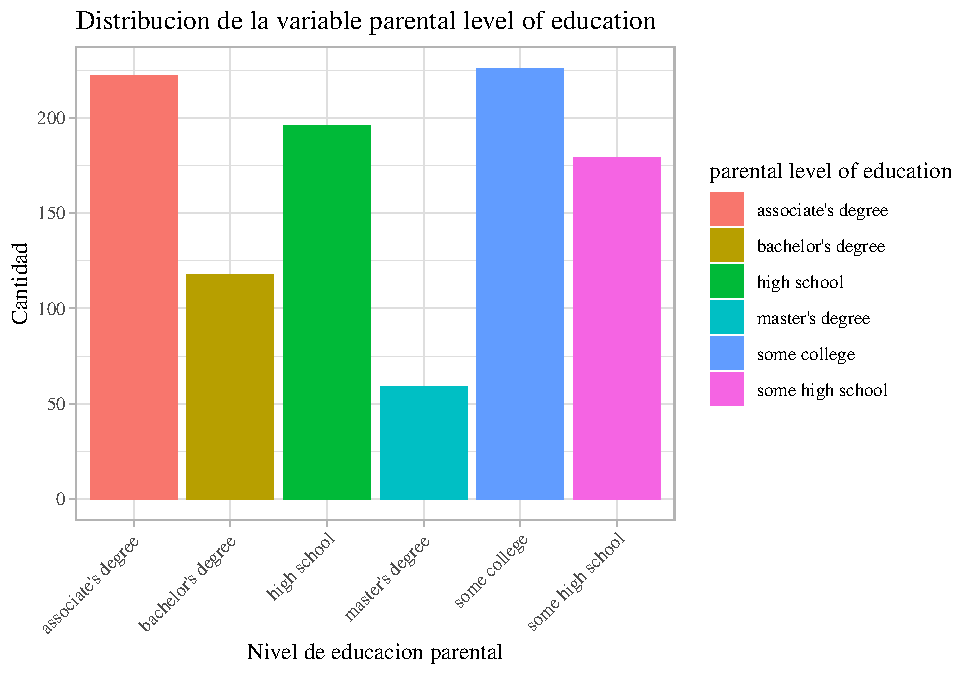
\includegraphics{Trabajo-Grupo-6.-Students-performance_files/figure-latex/unnamed-chunk-5-1} \end{center}

\begin{center}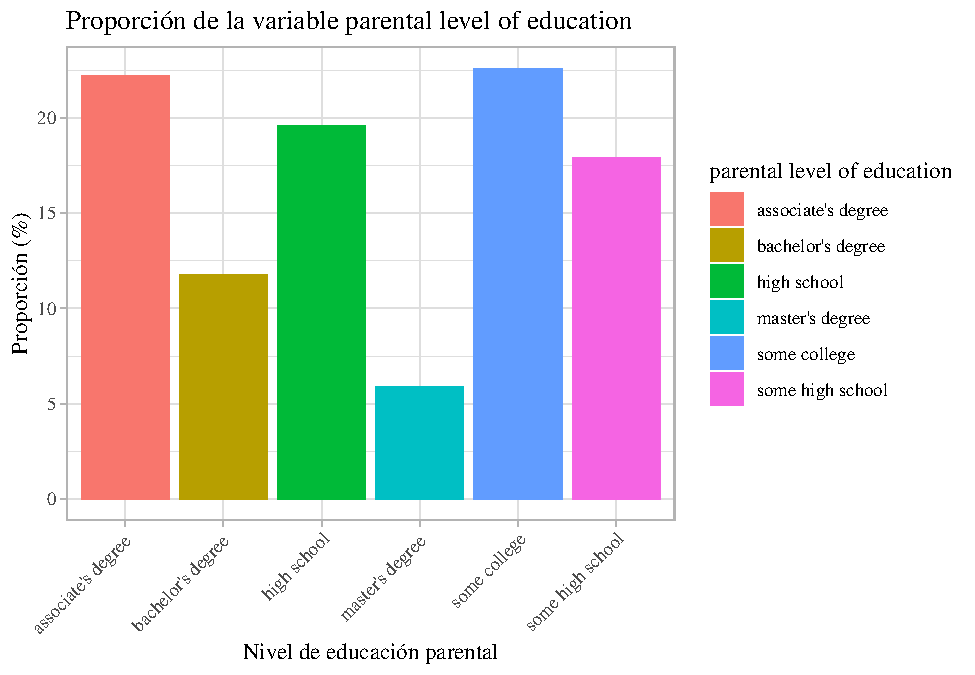
\includegraphics{Trabajo-Grupo-6.-Students-performance_files/figure-latex/unnamed-chunk-5-2} \end{center}

En el primer grafico se puede observar de manera visual, la distribución
de la variable parental level of education como ya fue mencionado
anteriormente. Además, en el segundo grafico se aprecia su distribución
porcentual.

A continuación, se hara lo mismo con la variable lunch.

\begin{center}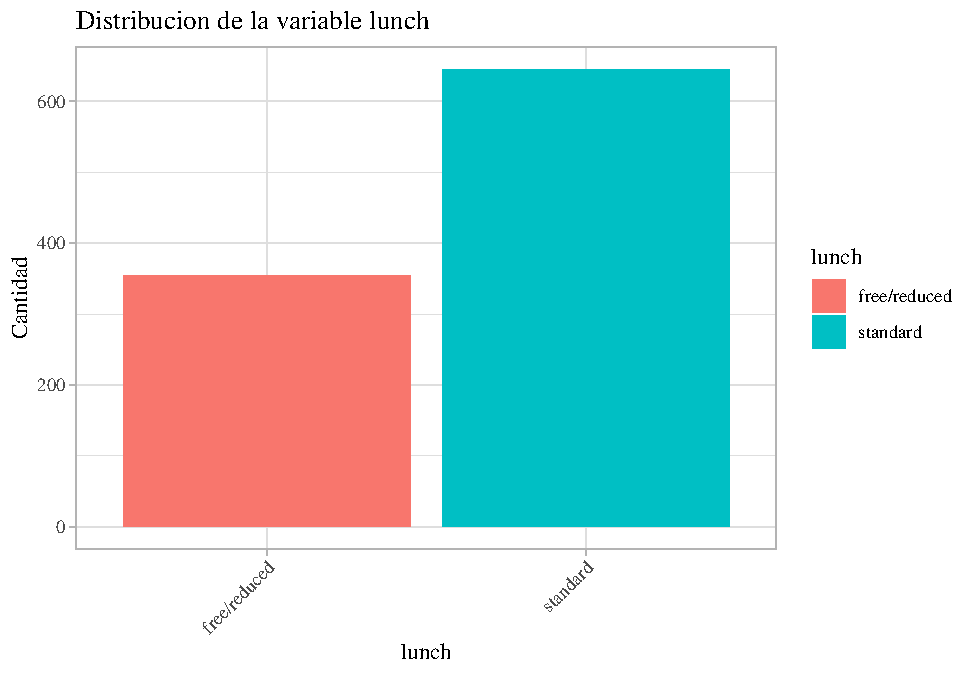
\includegraphics{Trabajo-Grupo-6.-Students-performance_files/figure-latex/unnamed-chunk-6-1} \end{center}

\begin{center}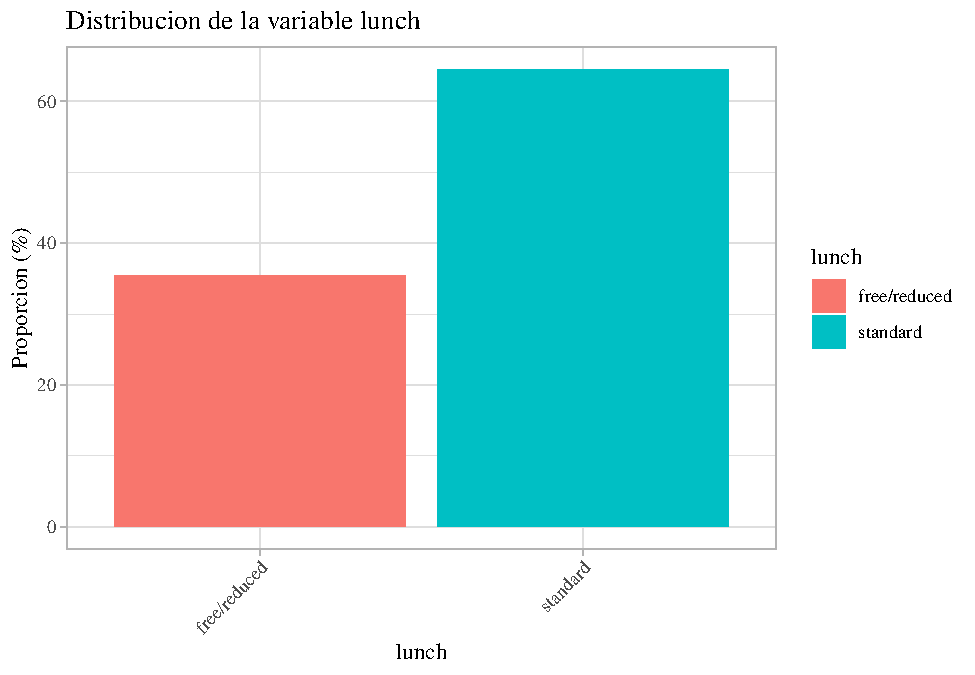
\includegraphics{Trabajo-Grupo-6.-Students-performance_files/figure-latex/unnamed-chunk-6-2} \end{center}

\section{Analisis Bivariante}\label{analisis-bivariante}

Para examinar si existe alguna clase de correlación entre las variables
``Nivel Educativo de los padres'' y ``Almuerzo'' en comparación a la
variable ``Desempeño'' analisaremos las proporciones, los cuartiles y la
asimetria y kurtosis de desempeño en relacion a las otras variables.

\begin{table}[!h]
\centering
\caption{\label{tab:tabla de frecuencias relativas porcentuales condicionales 1 }Frecuencias Relativas Condicionales Porcentuales por Nivel Educativo de los Padres}
\centering
\begin{tabular}[t]{lrrrrl}
\toprule
  & {}[9,32) & {}[32,55) & {}[55,78) & {}[78,100] & Sum\\
\midrule
\cellcolor{gray!10}{associate's degree} & \cellcolor{gray!10}{0.45} & \cellcolor{gray!10}{16.67} & \cellcolor{gray!10}{54.50} & \cellcolor{gray!10}{28.38} & \cellcolor{gray!10}{100}\\
bachelor's degree & 0.00 & 10.17 & 57.63 & 32.20 & 100\\
\cellcolor{gray!10}{high school} & \cellcolor{gray!10}{2.04} & \cellcolor{gray!10}{27.04} & \cellcolor{gray!10}{56.63} & \cellcolor{gray!10}{14.29} & \cellcolor{gray!10}{100}\\
master's degree & 0.00 & 11.86 & 47.46 & 40.68 & 100\\
\cellcolor{gray!10}{some college} & \cellcolor{gray!10}{1.77} & \cellcolor{gray!10}{12.83} & \cellcolor{gray!10}{59.73} & \cellcolor{gray!10}{25.66} & \cellcolor{gray!10}{100}\\
\addlinespace
some high school & 2.79 & 21.79 & 54.19 & 21.23 & 100\\
\bottomrule
\end{tabular}
\end{table}

En la tabla 4, se observa que los estudiantes cuyos padres tienen un
nivel educativo más alto, como ``bachelor's degree'' y ``master's
degree'', presentan un mayor porcentaje de estudiantes en los intervalos
de desempeño más altos. Por ejemplo, en el intervalo {[}78,100{]}, el
40.68\% de los estudiantes cuyos padres tienen un ``master's degree'' se
encuentran en este rango de alto desempeño, mientras que el 32.2\% de
los estudiantes con padres que tienen un ``bachelor's degree'' también
están en este intervalo, en comparación, solo el 14.29\% de los
estudiantes con padres que tienen un ``high school'' y el 21.23\% de
aquellos con padres que tienen un ``some high school'' alcanzan este
nivel de desempeño, esta tendencia sugiere una relación lineal directa
entre el nivel educativo de los padres y el desempeño académico de los
estudiantes, para una mejor visualización de esta relación, analizaremos
los cuartiles en la siguiente sección.

\begin{longtable}[t]{lrrr}
\caption{\label{tab:cuartiles}Cuartiles del Desempeño por Nivel Educativo de los Padres}\\
\toprule
parental level of education & Q1 & Q2 & Q3\\
\midrule
\cellcolor{gray!10}{associate's degree} & \cellcolor{gray!10}{58.67} & \cellcolor{gray!10}{69.67} & \cellcolor{gray!10}{79.00}\\
bachelor's degree & 64.08 & 71.16 & 80.67\\
\cellcolor{gray!10}{high school} & \cellcolor{gray!10}{53.92} & \cellcolor{gray!10}{65.00} & \cellcolor{gray!10}{72.67}\\
master's degree & 63.16 & 73.33 & 85.50\\
\cellcolor{gray!10}{some college} & \cellcolor{gray!10}{60.00} & \cellcolor{gray!10}{68.67} & \cellcolor{gray!10}{78.00}\\
\addlinespace
some high school & 55.66 & 66.67 & 76.50\\
\bottomrule
\end{longtable}

En la tabla 5, se observa que los estudiantes cuyos padres tienen un
nivel educativo más alto, como ``master's degree'' y ``bachelor's
degree'', presentan cuartiles más altos en comparación con aquellos
cuyos padres tienen un nivel educativo más bajo, como ``high school'' o
``some high school''. Por ejemplo, el Q3 (tercer cuartil) para
``master's degree'' es de 85.5 puntos, y para ``bachelor's degree'' es
de 80.67 puntos, en comparación, el Q3 para ``high school'' es de 72.67
puntos, y para ``some high school'' es de 76.5 puntos, esto significa
que el 75\% de los estudiantes con padres que tienen un ``master's
degree'' tienen un desempeño superior a 85.5 puntos, mientras que el
75\% de los estudiantes con padres que tienen un ``bachelor's degree''
tienen un desempeño superior a 80.67 puntos, por otro lado, el 75\% de
los estudiantes con padres que tienen un ``high school'' o ``some high
school'' tienen un desempeño superior a 72.67 puntos y 76.5 puntos,
respectivamente. Esta diferencia en los cuartiles, de nuevo, sugiere una
relación entre el nivel educativo de los padres y el desempeño académico
de los estudiantes, para una mejor visualización de esta relación, se
puede consultar el gráfico de cajas titulado ``Desempeño en función del
Nivel Educativo de los Padres''.

\begin{center}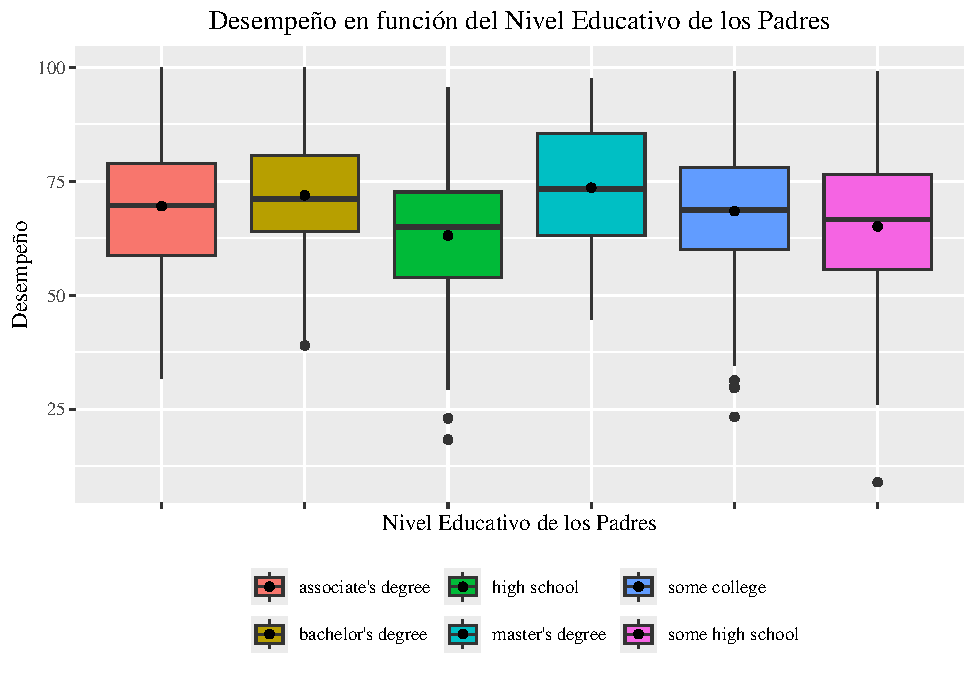
\includegraphics{Trabajo-Grupo-6.-Students-performance_files/figure-latex/grafico1-1} \end{center}

En este grafico podemos observar el comportamiento del desempeño según
el nivel educativo de los padres.

Primero que nada, es relevante entender la jerarquía entre cada nivel,
el cual es el siguiente: Master's \textgreater{} Bachellors
\textgreater{} Associate \textgreater{} Some college \textgreater{} High
school \textgreater{} Some high school.

Siguiendo esta jerarquía podemos establecer que los datos si presentan
una diferencia en el desempeño según el nivel educativo de los padres.
El mayor desempeño está asociado al Master's degree y cumple con la
jerarquía de nivel educativo ya mencionado de manera escalar, hasta
llegar a los dos últimos, a partir de esta instancia aquellos
estudiantes cuyos padres tienen solo algo de secundaria tuvieron mejor
desempeño comparado a los estudiantes con padres que si completaron la
secundaria.

\begin{table}[!h]
\centering
\caption{\label{tab:caculos basicos}Estadisticas Basicas del Desempeño por Nivel Educativo de los Padres}
\centering
\begin{tabular}[t]{lrrrrr}
\toprule
parental level of education & Promedio & D.Estandar & CV & Asimetria & Kurtosis\\
\midrule
\cellcolor{gray!10}{associate's degree} & \cellcolor{gray!10}{69.57} & \cellcolor{gray!10}{13.67} & \cellcolor{gray!10}{19.65} & \cellcolor{gray!10}{-0.10} & \cellcolor{gray!10}{-0.63}\\
bachelor's degree & 71.92 & 13.95 & 19.40 & -0.03 & -0.29\\
\cellcolor{gray!10}{high school} & \cellcolor{gray!10}{63.10} & \cellcolor{gray!10}{13.51} & \cellcolor{gray!10}{21.41} & \cellcolor{gray!10}{-0.39} & \cellcolor{gray!10}{0.19}\\
master's degree & 73.60 & 13.60 & 18.48 & -0.12 & -0.92\\
\cellcolor{gray!10}{some college} & \cellcolor{gray!10}{68.48} & \cellcolor{gray!10}{13.71} & \cellcolor{gray!10}{20.02} & \cellcolor{gray!10}{-0.38} & \cellcolor{gray!10}{0.25}\\
\addlinespace
some high school & 65.11 & 14.98 & 23.01 & -0.56 & 0.42\\
\bottomrule
\end{tabular}
\end{table}

De la tabla 6 podemos notar que mientras mayor es el ``Nivel Educativo
de los Padres'' mayor es la media de ``Desempeño'' de de los
estudiantes, por ejemplo, ``master's degree'' tiene 73.6 puntos en
promedio por estudiante y ``bachelor's degree'' tiene 71.92 puntos en
promedio por estudiante, mientras que ``some high school'' tiene 65.11
puntos en promedio por estudiante y ``high school'' tiene 63.10 puntos
en promedio por estudiante. El coeficiente de variación es más bajo para
los niveles educativos más altos, lo que indica que el desempeño es más
consistente en estos grupos, por ejemplo, ``master's degree'' tiene un
18.48\% de variación de notas por estudiante y ``bachelor's degree''
tiene un 19.4\% de variación de notas por estudiante, mientras que
``some high school'' tiene un 23.01\% de variación de notas por
estudiante y ``high school'' tiene un 21.41\% de variación de notas por
estudiante. En cuanto a la asimetría, los valores cercanos a cero
indican que la distribución de las notas es aproximadamente simétrica en
la mayoría de los grupos, aunque se observa un ligero sesgo hacia la
izquierda en algunos casos, como en ``high school'' (-0.39) y ``some
high school'' (-0.56), lo que sugiere que hay una mayor concentración de
estudiantes con calificaciones ligeramente más bajas en estos grupos.

El análisis de curtosis de Fisher revela diferencias en la distribución
de las notas de los hijos según el nivel educativo de los padres. Cuando
los padres poseen un master's degree (-0.92), associate's degree (-0.63)
o bachelor's degree (-0.29), las notas de los hijos muestran
distribuciones platicúrticas, lo que significa que hay menor
concentración alrededor de la media, mayor dispersión y ausencia de
valores extremos, lo que sugiere un desempeño académico heterogéneo. Por
el contrario, en hijos de padres con some high school (0.42), high
school (0.19) o some college (0.25), las distribuciones son
leptocúrticas, lo que significa que las notas estan agrupadas cerca de
la media y hay presencia moderada de valores extremos, lo que refleja
resultados más estandarizados, aunque con casos puntuales de desempeño
excepcional (alto o bajo). Entonces el nivel educativo de los padres se
asocia con patrones claros, a mayor formación académica parental
(master's degree, associate's degree, bachelor's degree), las notas de
los hijos tienden a dispersarse sin polarizarse, mientras que en niveles
educativos parentales básicos (some high school, high school, some
college), las notas se concentran en la media con cierta variabilidad en
extremos.

\begin{center}\includegraphics{Trabajo-Grupo-6.-Students-performance_files/figure-latex/histogramasa1-1} \end{center}

\begin{center}\includegraphics{Trabajo-Grupo-6.-Students-performance_files/figure-latex/histogramasa2-1} \end{center}

\begin{center}\includegraphics{Trabajo-Grupo-6.-Students-performance_files/figure-latex/histogramasa3-1} \end{center}

\begin{center}\includegraphics{Trabajo-Grupo-6.-Students-performance_files/figure-latex/histogramasa4-1} \end{center}

\begin{center}\includegraphics{Trabajo-Grupo-6.-Students-performance_files/figure-latex/histogramasa5-1} \end{center}

\begin{center}\includegraphics{Trabajo-Grupo-6.-Students-performance_files/figure-latex/histogramasa6-1} \end{center}

\begin{table}[!h]
\centering
\caption{\label{tab:tabla de frecuencias relativas porcentuales condicionales 2 }Frecuencias Relativas Condicionales Porcentuales por Calidad de Almuerzo}
\centering
\begin{tabular}[t]{lrrrrl}
\toprule
  & {}[9,32) & {}[32,55) & {}[55,78) & {}[78,100] & Sum\\
\midrule
\cellcolor{gray!10}{free/reduced} & \cellcolor{gray!10}{3.10} & \cellcolor{gray!10}{27.04} & \cellcolor{gray!10}{55.21} & \cellcolor{gray!10}{14.65} & \cellcolor{gray!10}{100}\\
standard & 0.47 & 12.56 & 56.43 & 30.54 & 100\\
\bottomrule
\end{tabular}
\end{table}

En la tabla 7 podemos observar que los estudiantes que reciben un
almuerzo ``standard'' tienen un porcentaje mayor de estudiantes en los
intervalos de desempeño más altos en proporción que los que reciben un
almuerzo ``free/reduced'', por ejemplo, en el intervalo {[}78,100{]},
hay un 30,54\% de estudiantes que consumen el almuerzo ``standard'' y
solo un 14,65\% de estudiantes que consumen el almuerzo
``free/reduced'', esto sugiere que la calidad del almuerzo está
relacionada con un mejor rendimiento académico, pasemos analizar mejor
esto mediante cuartiles.

\begin{table}[!h]
\centering
\caption{\label{tab:cuartiles2}Cuartiles del Desempeño Calidad de Almuerzo}
\centering
\begin{tabular}[t]{lrrr}
\toprule
lunch & Q1 & Q2 & Q3\\
\midrule
\cellcolor{gray!10}{free/reduced} & \cellcolor{gray!10}{52.84} & \cellcolor{gray!10}{62.67} & \cellcolor{gray!10}{72.50}\\
standard & 62.33 & 71.33 & 79.67\\
\bottomrule
\end{tabular}
\end{table}

La tabla 8 muestra que los estudiantes que reciben un almuerzo
``standard'' tienen un desempeño más alto en comparación con los que
reciben un almuerzo ``free/reduced'', ya que los estudiantes con
almuerzo estandar tienen un ``Desempeño'' superior al de los estudiantes
con almuerzos ``free/reduced'', por ejemplo, el Q3 (tercer cuartil) para
``standard'' es de 79.67 puntos, mientras que para ``free/reduced'' es
de 72.50 puntos, esto indica que el 75\% de los estudiantes con almuerzo
``standard'' tienen un desempeño superior a 79.67 puntos, mientras que
el 75\% de los estudiantes con almuerzo ``free/reduced'' tienen un
desempeño superior a 72.50 puntos, todo esto se puede observar mucho
mejor en el grafico ``Desempeño en función de la Calidad de los
Almuerzos''.

\begin{center}\includegraphics{Trabajo-Grupo-6.-Students-performance_files/figure-latex/grafico2-1} \end{center}

En este simple grafico podemos observar de manera clara que los
estudiantes con un almuerzo estándar (standard) tuvieron un mejor
desempeño que aquellos con un almuerzo reducido.

\begin{table}[!h]
\centering
\caption{\label{tab:calculos basicos2}Estadisticas Basicas del Desempeño por Calidad de Almuerzo}
\centering
\begin{tabular}[t]{lrrrrr}
\toprule
lunch & Promedio & D.Estandar & CV & Asimetria & Kurtosis\\
\midrule
\cellcolor{gray!10}{free/reduced} & \cellcolor{gray!10}{62.20} & \cellcolor{gray!10}{14.46} & \cellcolor{gray!10}{23.25} & \cellcolor{gray!10}{-0.31} & \cellcolor{gray!10}{0.22}\\
standard & 70.84 & 13.19 & 18.62 & -0.19 & -0.19\\
\bottomrule
\end{tabular}
\end{table}

La Tabla 9 muestra que los estudiantes con almuerzo ``standard'' tienen
un promedio de desempeño (70.84 puntos), mayor al de los estudiantes con
almuerzo ``free/reduced'' (62.20 puntos). Además, el coeficiente de
variación (CV) es menor para los estudiantes con almuerzo ``standard''
(18.62\%) en comparación con los que tienen almuerzo ``free/reduced''
(23.25\%), lo que indica que el desempeño es más consistente y menos
disperso en el primer grupo. En cuanto a la asimetría, ambos grupos
presentan un ligero sesgo hacia la izquierda, es decir, una mayor
concentración de estudiantes con calificaciones ligeramente más bajas,
más los estudiantes con almuerzo ``free/reduced'' (con -0.31) que los
que consumen el almuerzo ``standard'' (con -0.19)

Por otro lado, la curtosis muestra que el grupo con almuerzo
``standard'' tiene un valor de -0.19, lo que indica una distribución
ligeramente platicúrtica, con menor concentración alrededor de la media
y ausencia de valores extremos. En contraste, el grupo con almuerzo
``free/reduced'' presenta una curtosis de 0.22, lo que sugiere una
distribución ligeramente leptocúrtica, con mayor concentración de notas
alrededor de la media y una presencia moderada de valores extremos, esto
implica que, aunque el desempeño es más consistente en el grupo con
almuerzo ``standard'', también hay una mayor variabilidad en los
extremos en el grupo con almuerzo ``free/reduced''.

\begin{center}\includegraphics{Trabajo-Grupo-6.-Students-performance_files/figure-latex/histogramasb1-1} \end{center}

\begin{center}\includegraphics{Trabajo-Grupo-6.-Students-performance_files/figure-latex/histogramasb2-1} \end{center}

\section{Comparación de las Tres Variables en
Conjunto}\label{comparaciuxf3n-de-las-tres-variables-en-conjunto}

\begin{center}\includegraphics{Trabajo-Grupo-6.-Students-performance_files/figure-latex/grafico3-1} \end{center}

Finalmente, llegamos a la parte más importante del trabajo, el grafico
que relaciona las 3 variables analizadas. Es una combinación de dos
gráficos ya mencionados.

Primero que nada, hay 5 pares de figuras, la primera está identificada
con el color rojo y la segunda con el color azul, de izquierda a
derecha. Luego cada color representa los distintos niveles de educación
de los padres.

En este grafico podemos ver claramente que los estudiantes con un
almuerzo estándar tuvieron un mejor desempeño que los demás. También, se
ve la diferencia de desempeño según el nivel educativo parental,
mientras mayor sea, mejor el desempeño de los estudiantes.

En resumen, la información presentada es la misma que la de los gráficos
anteriores pero de manera conjunta, lo cual representa de manera breve y
concisa el análisis realizado en este trabajo.

\#Conclusión

A lo largo de este trabajo, se ha analizado la relación entre el nivel
educativo de los padres y la calidad del almuerzo de los estudiantes con
su desempeño académico, utilizando datos de un grupo representativo de
estudiantes estadounidenses. Los resultados obtenidos respaldan la
hipótesis inicial de que ambas variables tienen un impacto significativo
en el rendimiento académico de los estudiantes. Los análisis realizados
muestran una clara relación entre el nivel educativo de los padres y el
desempeño académico de los estudiantes. En general, los estudiantes
cuyos padres tienen un nivel educativo más alto tienden a obtener
calificaciones más altas en comparación con aquellos cuyos padres tienen
un nivel educativo más bajo. Esto se evidencia en los cuartiles, donde
los estudiantes con padres más educados presentan valores más altos, lo
que indica un mejor desempeño en todos los niveles de distribución.
Además, el coeficiente de variación es más bajo en los grupos con padres
con un mayor nivel de estudio, lo que sugiere que el desempeño es más
consistente y menos disperso en estos grupos.

Estos resultados están en concordancia con los antecedentes teóricos,
que sugieren que los padres con mayor nivel educativo tienden a invertir
más tiempo en el desarrollo académico de sus hijos, fomentan una cultura
de estudio y proporcionan un entorno más propicio para el aprendizaje,
reforzando la idea de que el nivel educativo de los padres es un factor
determinante en el éxito académico de los estudiantes. En cuanto a la
calidad del almuerzo, los resultados indican que los estudiantes que
reciben un almuerzo ``standard'' tienen un mejor desempeño académico en
comparación con aquellos que reciben un almuerzo ``free/reduced''. En
términos generales, los estudiantes con almuerzo ``standard'' presentan
una mayor proporción en los intervalos de desempeño más altos, mientras
que aquellos con almuerzo ``free/reduced'' tienden a concentrarse en los
intervalos de desempeño más bajos. Los cuartiles también reflejan esta
tendencia, mostrando que los estudiantes con almuerzo ``standard''
tienen un desempeño superior en todos los percentiles analizados.

Estos resultados respaldan la hipotesis de que una alimentación adecuada
y balanceada tiene un impacto positivo en la capacidad cognitiva, la
concentración y el rendimiento académico de los estudiantes. Una
nutrición deficiente, por otro lado, puede afectar negativamente el
desempeño escolar, lo que subraya la importancia de programas de
alimentación escolar que aseguren una dieta equilibrada para todos los
estudiantes. Al comparar ambas variables, se observa que el nivel
educativo de los padres tiene un impacto más pronunciado en el desempeño
académico que la calidad del almuerzo. Sin embargo, ambas variables son
significativas y están interrelacionadas. Los estudiantes con padres más
educados tienen más probabilidades de acceder a una alimentación de
mejor calidad, lo que a su vez refuerza su rendimiento académico. Esto
sugiere que las políticas educativas y sociales deben abordar ambas
dimensiones para maximizar el impacto en el desempeño estudiantil.

Los hallazgos de este estudio ofrecen evidencias que sugieren que sería
positivo replantear ciertas políticas en el ámbito educativo y social.
En primer lugar, es fundamental implementar programas que apoyen a las
familias con menores niveles educativos, brindándoles herramientas y
recursos para fomentar el éxito académico de sus hijos. Esto podría
incluir talleres para padres, programas de tutoría y acceso a materiales
educativos. En segundo lugar, es crucial garantizar que todos los
estudiantes tengan acceso a una alimentación adecuada, ya sea a través
de programas de almuerzos escolares subsidiados o iniciativas que
promuevan una nutrición balanceada.

Es importante reconocer que este estudio tiene limitaciones. En primer
lugar, los datos utilizados son de un grupo específico de estudiantes
estadounidenses, por lo que los resultados pueden no ser generalizables
a otros contextos culturales o socioeconómicos. Además, el estudio no
profundiza en las razones específicas detrás de las relaciones
observadas, como el tiempo que los padres dedican a sus hijos o los
hábitos alimenticios específicos. Futuras investigaciones podrían
explorar estas dimensiones con mayor detalle, utilizando metodologías
cualitativas y cuantitativas complementarias.

En conclusión, este estudio confirma que tanto el nivel educativo de los
padres como la calidad del almuerzo de los estudiantes son factores
clave que influyen en el rendimiento académico. Ambos aspectos deben ser
considerados en el diseño de políticas educativas y sociales que busquen
mejorar el desempeño escolar y, en última instancia, contribuir al
desarrollo socioeconómico de las comunidades. Un enfoque integral que
combine el apoyo familiar y la nutrición adecuada puede ser la clave
para reducir las brechas educativas y promover un entorno más equitativo
y propicio para el aprendizaje.

\end{document}
